\section{Heterogeneous Catalysis}

Detail found in Corentin thesis and dutch guy thesis

\subsection{Mechanisms}

In heterogeneous catalysis, two mechanisms are generally considered : the Langmuir–Hinshelwood mechanism [44, 45, 46] and the Eley–Rideal mechanism [47]. In the first mechanism both reactants are adsorbed at the surface of the catalyst, react at the surface and then happen the desorption of the product. In Eley–Rideal mechanism, only one of the reactant is adsorbed while the other one reacts with it directly from the gas phase. The first mechanism (Langmuir–Hinshelwood) appears to be generally preferred [48] (Fig. 1.1).

Last meachanism is Mars - Van Krevelen (MvK) mechanism

The overall heterogeneous catalytic reaction generally consists of a series of elementary
steps : adsorption of the reactants, diffusion on the surface, breaking of reactants bonds, creation of new bonds to form products and finally desorption of these new chemicals. Catalysts are usually complex systems in powder form (presenting different surface orientation, i.e. facets) coupled with promoters (chemicals that improve the catalytic activity). It is therefore difficult to provide a molecular-level understanding of such processes. Model catalysts can therefore be used to simplify the investigation. A well-built theory has been proposed by Hammer and Nørskov [49] and lays down the basic rules behind catalysis. Some key parameters are used to rationalize and describe a catalytic process and catalysts performances. More recent approaches involving the use of machine learning can help predict the key descriptors for catalysis [50, 51]. Hammer and Nørskov theory is more of a model theoretical approach that could be experimentally questioned by model catalysts.

Catalysis is described by key parameters such as the stability (the propensity of the catalyst to stay unchanged after the reaction), the activity and the turn-over frequency (TOF, number of mole of reactant that can be converted per mole of catalyst over time), the selectivity (for example targeting the production of one particular isomer), the propensity to deactivation of the catalyst (for instance due to its oxidation). Depending on the chemical reaction, one wishes to have an active catalyst that is very stable and very selective towards a unique product, and doing so for a long time. However, it is difficult to meet all the requirements at once. A high activity is unfortunately often linked to a poor selectivity

Hammer and Nørskov [49] have compiled and provided a well-built theory of adsorbates
surface interactions for simple transition metals. As shown in Fig. 1.2, the model predicts that as the d-band of the metal shifts up towards the Fermi level (the filling of the band is kept fixed so that as the center of the d-band is shifted up, the band width decreases), the electron density of states of the adsorbate is modified and antibonding states appear above the Fermi level. Therefore they are empty and the bonds become stronger as the number of empty antibonding states increases. In short, the closer to the Fermi level and the narrower the d-band, the stronger the bonding i.e. the chemisorption.

This model seems to work fine for simple transition metals (3d, 4d and 5d) [38, 39] for chemisorption (e.g. oxygen adsorption [49]) and also for molecular dissociation (e.g. CO
dissociation [53], NO dissociation on Ru(0001) [42]). A clear linear correlation between adsorption energies and d-band position is determined both experimentally and theoretically. This is similar to the Brønsted-Evans-Polanyi linear relation between the activation and reaction energies. In the case of a monolayer of a transition metal over a substrate, a similar behavior is observed and the model still works fine (e.g. 5d metals on Pt(111) [54])


Role of strain : 

\cite{Kitchin2004}

\cite{Mavrikakis1998}

We define a system where a (metal) sample, consisting of a surface and a bulk is in contact with a gaseous environment.




\subsubsection{Materials}

\subsubsection{Conditions}

This reaction is considered as a classic example of a strongly exothermic, heterogeneous, catalytic reaction [4]. Due to the very fast kinetics of oxidation reactions, a direct experimental investigation of several reaction steps is difficult at realistic conditions.

nitrous oxide is a powerful oxidiser similar to molecular oxygen. 

Selectivity to nitrous oxide at low temperature was reported in the following order: $Pt > Pd > Ni > Fe > W > Ti $[6].

N2O selectivity for us ?

NH3 oxidation requires surface sites for the adsorption of two ammonia molecules and two oxygen atoms.

Furthermore, the importance of availability of oxygen vacant sites near N-containing adspecies was demonstrated by the decrease of the reaction rate when a surface oxide was formed [31–33].
Finally, adsorbed oxygen did not block the ammonia adsorption [12]. All these facts led to the conclusion that a dual-site mechanism is operative. A similar conclusion on the reaction mechanism was made for ammonia oxidation on a supported ruthenium catalyst [34].

\begin{figure}[ht]
    \centering
    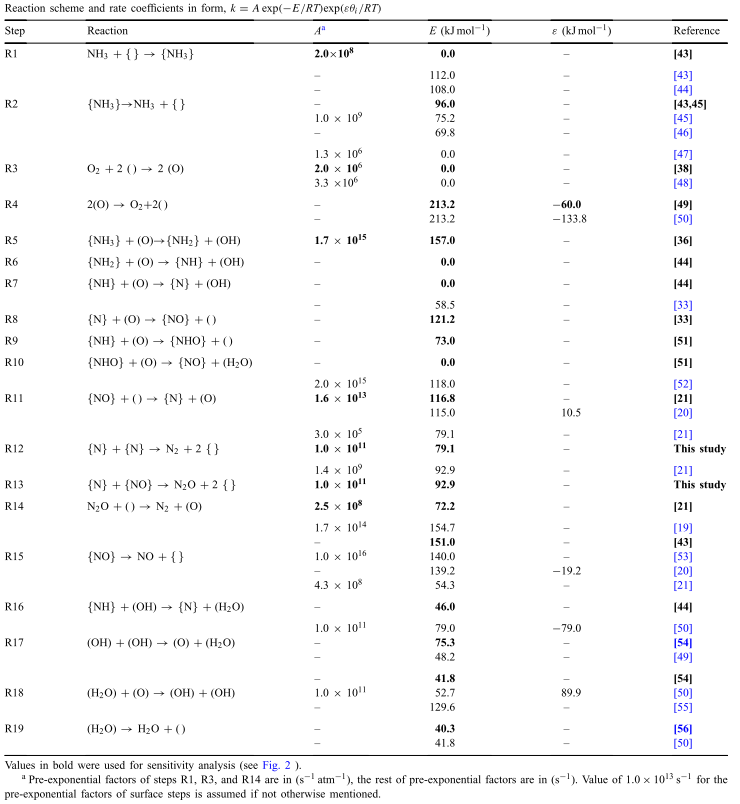
\includegraphics[width=\textwidth]{Images/ReactionScheme.png}
    \caption{\cite{Rebrov2002}}
    \label{fig:my_label}
\end{figure}

Relation to nanoparticle size
It was also reported that the stoichiometry of oxygen chemisorption increases by a factor 2.7 with increasing platinum crystallite size. This could also lead to an increase of the reaction rate if the oxygen adsorption is the rate-determining step in this system.

\subsection{Particle-Size Effect in Catalytic Oxidation Over Pt Nanoparticles}

Alexandr Yu. Stakheev, ..., Valerii I. Bukhtiyarov, in Advanced Nanomaterials for Catalysis and Energy, 2019

Relationships between turnover frequency and the size of supported Pt clusters are discussed for oxidation of hydrocarbons, CO, and NO by molecular oxygen. Analysis of the experimental data indicates that TOF tends to increase for bigger platinum particles. This tendency is particularly pronounced for the nanoparticles smaller than 4–5 nm. According to the most realistic models, the observed tendency stems from the deactivation of edge, corner, and neighboring atoms by two processes: (1) strong oxygen adsorption on edge and corner atoms with high degree of coordinative unsaturation, and (2) oxidation of Pt to PtOx, which is facilitated over undercoordinated sites. As the metal clusters grow in size, the fraction of undercoordinated edge and corner atoms decreases leading to the increase in experimentally observed TOF.


The increase of supported platinum particle size led also
to considerable changes in selectivity in the ammonia oxidation over a Pt/Al2O3 catalyst [7,22,26]. Large crystallites of 15.5 nm, for which over 98\% of the surface atoms are plane atoms [28], exhibited low selectivity to nitrogen formation. Selectivity to nitrogen increased with decreasing platinum loading

\subsection{Stability}

The turnover frequency TOF quantifies the specific activity of a catalytic centre for a special reaction under defined reaction conditions by the number of molecular reactions or catalytic cycles occurring at the centre per unit time. For heterogeneous catalysts the number of active centres is derived usually from sorption methods.

Separate from the TOF, evaluating the catalytic activity, the turnover number (TON) value is an important parameter to evaluate the stability of the catalyst. In homogeneous and heterogeneous catalysis, the TON is a dimensionless number,24,25 which is defined as the number of the molecules produced per catalytic site before deactivation under given reaction conditions. That is to say, the catalyst can achieve the total number of turnovers until it is totally dead, regardless of the reaction time.26 In this respect, an ideal catalyst should have an infinite TON. Thus, the TON represents the maximum yield of products attained from an active catalytic site up to the decay of activity for a specific reaction. The TON of a catalyst for water oxidation is calculated according to Eq. (5):


\subsection{Linking strain and reactivity}

Hammer and Noskrov blabla
